\reviewexercisesheader{}

% 31 - gaming_distracted_eating_intake

\eoce{\qt{Gaming and distracted eating, Part I\label{gaming_distracted_eating_intake}}
A group of researchers are interested in the possible effects of distracting 
stimuli during eating, such as an increase or decrease in the amount of food 
consumption. To test this hypothesis, they monitored food intake for a group of 
44 patients who were randomized into two equal groups. The treatment group ate 
lunch while playing solitaire, and the control group ate lunch without any 
added distractions. Patients in the treatment group ate 52.1 grams of biscuits, 
with a standard deviation of 45.1 grams, and patients in the control group ate 
27.1 grams of biscuits, with a standard deviation of 26.4 grams. Do these data 
provide convincing evidence that the average food intake (measured in amount of 
biscuits consumed) is different for the patients in the treatment group? Assume 
that conditions for inference are satisfied. \footfullcite{Oldham:2011}
}{}

% 32 - gaming_distracted_eating_recall

\eoce{\qt{Gaming and distracted eating, Part II\label{gaming_distracted_eating_recall}} 
The researchers from Exercise~\ref{gaming_distracted_eating_intake} also 
investigated the effects of being distracted by a game on how much people eat. 
The 22 patients in the treatment group who ate their lunch while playing 
solitaire were asked to do a serial-order recall of the food lunch items they 
ate. The average number of items recalled by the patients in this group was 4.
9, with a standard deviation of 1.8. The average number of items recalled by 
the patients in the control group (no distraction) was 6.1, with a standard 
deviation of 1.8. Do these data provide strong evidence that the average number 
of food items recalled by the patients in the treatment and control groups are 
different?
}{}

% 33 - sample_size_pairing

\eoce{\qt{Sample size and pairing\label{sample_size_pairing}} Determine if the 
following statement is true or false, and if false, explain your reasoning: If 
comparing means of two groups with equal sample sizes, always use a paired test.
}{}

% 34 - college_credits

\eoce{\qt{College credits\label{college_credits}}
A college counselor is interested in 
estimating how many credits a student typically enrolls
in each semester.
The counselor decides to randomly sample 100 students
by using the registrar's 
database of students.
The histogram below shows the distribution of the number 
of credits taken by these students.
Sample statistics for this distribution are 
also provided.\\
\begin{minipage}[c]{0.1\textwidth}
\ 
\end{minipage}
\begin{minipage}[c]{0.5\textwidth}
\begin{center}
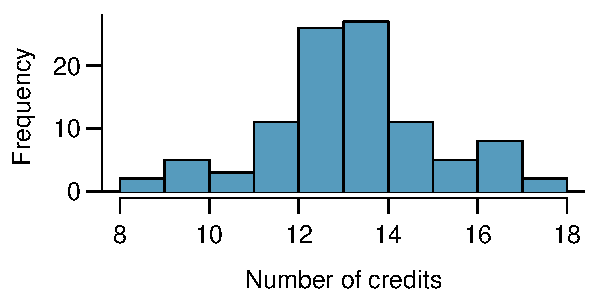
\includegraphics[width=\textwidth]{ch_inference_for_means/figures/eoce/college_credits/college_credits_hist.pdf}
\end{center}
\end{minipage}
\begin{minipage}[c]{0.32\textwidth}
\begin{center}
\begin{tabular}{l|r l}
Min     & 8 \\
Q1      & 13 \\
Median  & 14 \\
Mean    & 13.65 \\
SD      & 1.91 \\
Q3      & 15 \\
Max     & 18 \\
\end{tabular}
\end{center}
\end{minipage}
\begin{parts}
\item What is the point estimate for the average
number of credits taken per semester by students at this college?
What about the median?
\item What is the point estimate for the standard deviation
of the number of credits taken per semester by students at
this college?
What about the IQR?
\item Is a load of 16 credits unusually high for this college?
What about 18 credits?
Explain your reasoning.
\item The college counselor takes another
random sample of 100 students and this 
time finds a sample mean of 14.02 units.
Should she be surprised that this sample
statistic is slightly different than the
one from the original sample? 
Explain your reasoning.
\item
The sample means given above are point estimates
for the mean number of 
credits taken by all students at that college.
What measures do we use to 
quantify the variability of this estimate?
Compute this quantity using the data 
from the original sample.
\end{parts}
}{}

% 35 - hen_eggs

\eoce{\qt{Hen eggs\label{hen_eggs}} The distribution of the number of eggs laid 
by a certain species of hen during their breeding period has a mean of 35 eggs 
with a standard deviation of 18.2. Suppose a group of researchers 
randomly samples 45 hens of this species, counts the number of eggs laid 
during their breeding period, and records the sample mean. They repeat 
this 1,000 times, and build a distribution of sample 
means. 
\begin{parts}
\item What is this distribution called? 
\item Would you expect the shape of this distribution to be symmetric, right 
skewed, or left skewed? Explain your reasoning.
\item Calculate the variability of this distribution and state the appropriate 
term used to refer to this value.
\item Suppose the researchers' budget is reduced and they are only able to 
collect random samples of 10 hens. The sample mean of the number of eggs is 
recorded, and we repeat this 1,000 times, and build a new distribution of sample 
means. How will the variability of this new distribution compare to the 
variability of the original distribution?
\end{parts}
}{}

% 36 - forest_mgmt_tree_growth

\eoce{\qt{Forest management\label{forest_mgmt_tree_growth}}
Forest rangers wanted to better understand the rate
of growth for younger trees in the park.
They took measurements of a random sample of 50 young trees
in 2009 and again measured those same trees in 2019.
The data below summarize their measurements,
where the heights are in feet:
\begin{center}
\begin{tabular}{l c c c}
\hline
          & 2009   & 2019  & Differences\\
\hline  
$\bar{x}$ & 12.0  & 24.5  & 12.5 \\
$s$       & 3.5   & 9.5   & 7.2 \\
$n$       & 50    & 50    & 50 \\
\hline
\end{tabular}
\end{center}
Construct a 99\% confidence interval for the
average growth of (what had been) younger trees
in the park over 2009-2019.
}{}

% 37 - exclusive_relationships

\eoce{\qt{Exclusive relationships\label{exclusive_relationships}} A survey conducted 
on a reasonably random sample of 203 undergraduates asked, among many other 
questions, about the number of exclusive relationships these students have been 
in. The histogram below shows the distribution of the data from this sample. 
The sample average is 3.2 with a standard deviation of 1.97.
\begin{center}
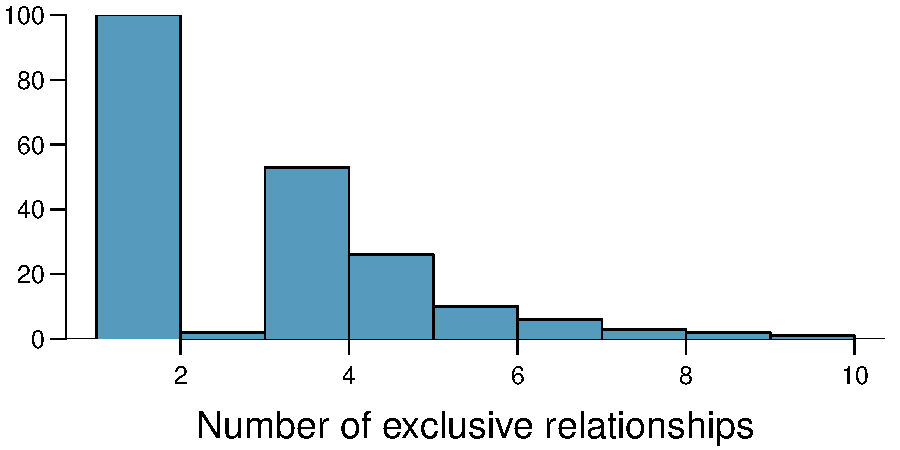
\includegraphics[width=0.6\textwidth]{ch_inference_for_means/figures/eoce/exclusive_relationships/exclusive_relationships_rel_hist.pdf}
\end{center}
Estimate the average number of exclusive relationships Duke students have been 
in using a 90\% confidence interval and interpret this interval in context. 
Check any conditions required for inference, and note any assumptions you must 
make as you proceed with your calculations and conclusions.
}{}

% 38 - age_at_first_marriage_intro

\eoce{\qt{Age at first marriage, Part I\label{age_at_first_marriage_intro}} 
The National Survey of Family Growth conducted by the Centers for Disease 
Control gathers information on family life, marriage and divorce, pregnancy, 
infertility, use of contraception, and men's and women's health. One of the 
variables collected on this survey is the age at first marriage. The histogram 
below shows the distribution of ages at first marriage of 5,534 randomly sampled 
women between 2006 and 2010. The average age at first marriage among these women 
is 23.44 with a standard deviation of 4.72.\footfullcite{data:nsfg:2010}
\begin{center}
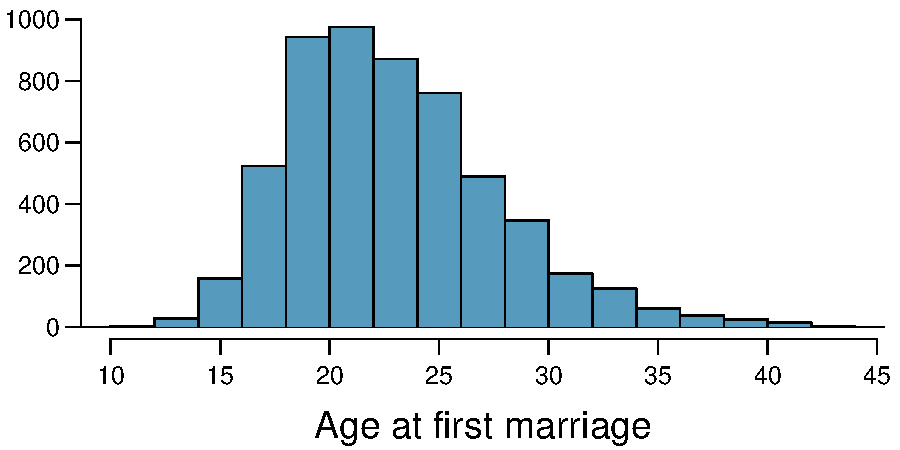
\includegraphics[width=0.6\textwidth]{ch_inference_for_means/figures/eoce/age_at_first_marriage_intro/age_at_first_marriage_intro_hist.pdf}
\end{center}
Estimate the average age at first marriage of women using a 95\% confidence 
interval, and interpret this interval in context. Discuss any relevant 
assumptions.
}{}

% 39 - online_communication

\eoce{\qt{Online communication\label{online_communication}} A study suggests that the 
average college student spends 10 hours per week communicating with others 
online. You believe that this is an underestimate and decide to collect your 
own sample for a hypothesis test. You randomly sample 60 students from your 
dorm and find that on average they spent 13.5 hours a week communicating with 
others online. A friend of yours, who offers to help you with the hypothesis 
test, comes up with the following set of hypotheses. Indicate any errors you see.
\begin{align*}
H_0&: \bar{x} < 10~hours \\
H_A&: \bar{x} > 13.5~hours
\end{align*}
}{}

% 40 - age_at_first_marriage_hyp_errors

\eoce{\qt{Age at first marriage, Part II\label{age_at_first_marriage_hyp_errors}} Exercise~\ref{age_at_first_marriage_intro} presents the results 
of a 2006 - 2010 survey showing that the average age of women at first marriage 
is 23.44.
Suppose a social scientist thinks this value has changed 
since the survey was taken.
Below is how she set up her hypotheses.
Indicate any errors you see.
\begin{align*}
H_0&: \bar{x} \neq 23.44~years~old \\
H_A&: \bar{x} = 23.44~years~old
\end{align*}
}{}

% 41 - friday_13th_traffic

\eoce{\qt{Friday the 13$^{\text{th}}$, Part I\label{friday_13th_traffic}} In the 
early 1990's, researchers in the UK collected data on traffic flow, number of 
shoppers, and traffic accident related emergency room admissions on Friday the 
13$^{\text{th}}$ and the previous Friday, Friday the 6$^{\text{th}}$. The 
histograms below show the distribution of number of cars passing by a specific 
intersection on Friday the 6$^{\text{th}}$ and Friday the 13$^{\text{th}}$ for 
many such date pairs. Also given are some sample statistics, where the 
difference is the number of cars on the 6th minus the number of cars on the 13th.\footfullcite{Scanlon:1993}
\begin{center}
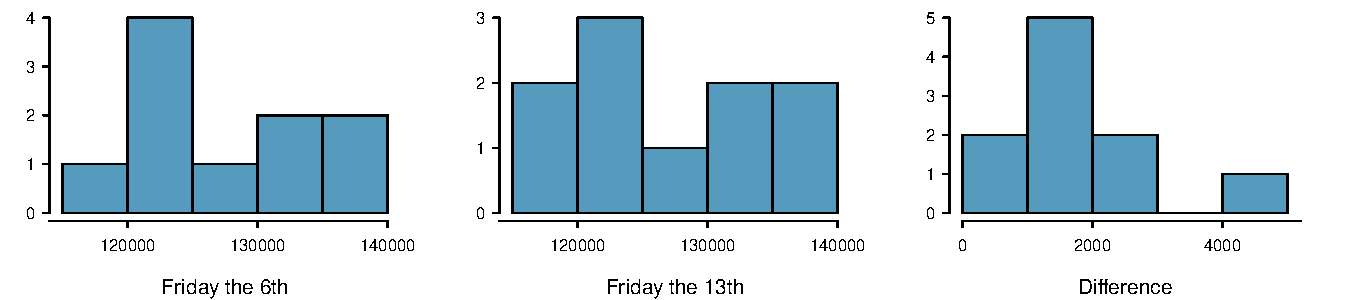
\includegraphics[width=\textwidth]{ch_inference_for_means/figures/eoce/friday_13th_traffic/friday_13th_traffic_hist} \\
$\:$ \\
{\small
\begin{tabular}{l c c c}
\hline
        & 6$^{\text{th}}$   & 13$^{\text{th}}$  & Diff.\\
\hline  
$\bar{x}$   &128,385            & 126,550       & 1,835 \\
$s$     &7,259          & 7,664         & 1,176 \\
$n$     &10             & 10                & 10 \\
\hline
\end{tabular}
}
\end{center}
\begin{parts}
\item Are there any underlying structures in these data that should be 
considered in an analysis? Explain.
\item What are the hypotheses for evaluating whether the number of people out 
on Friday the 6$^{\text{th}}$ is different than the number out on Friday the 
13$^{\text{th}}$?
\item Check conditions to carry out the hypothesis test from part~(b).
\item Calculate the test statistic and the p-value.
\item What is the conclusion of the hypothesis test?
\item Interpret the p-value in this context.
\item What type of error might have been made in the conclusion of your test? 
Explain.
\end{parts}
}{}

% 42 - friday_13th_accident

\eoce{\qt{Friday the 13$^{\text{th}}$, Part II\label{friday_13th_accident}} \videosolution{friday_13_accident_solution} 
The Friday the $13^{th}$ study reported in
Exercise~\ref{friday_13th_traffic} also provides data on traffic
accident related emergency room admissions.
The distributions of these counts from Friday the 6$^{\text{th}}$ and
Friday the 13$^{\text{th}}$ are shown below for six such paired dates
along with summary statistics.
You may assume that conditions for inference are met.
\begin{center}
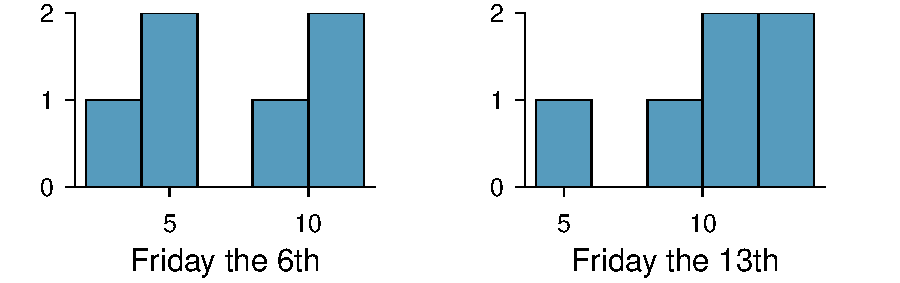
\includegraphics[width=0.74\textwidth]{ch_inference_for_means/figures/eoce/friday_13th_accident/friday_13th_accident_hist} \\
$\:$ \\
\begin{minipage}[c]{0.36\textwidth}
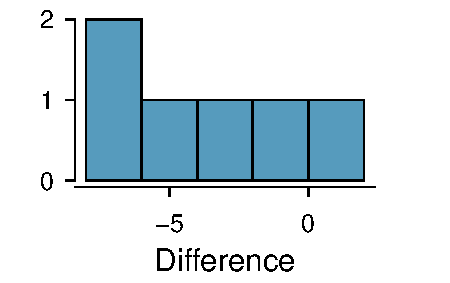
\includegraphics[width=\textwidth]{ch_inference_for_means/figures/eoce/friday_13th_accident/friday_13th_accident_hist_diff}
\end{minipage}
\begin{minipage}[c]{0.36\textwidth}
\ \ \begin{tabular}{l c c c}
\hline
        & 6$^{\text{th}}$   & 13$^{\text{th}}$  & diff\\
\hline  
Mean    &7.5                & 10.83             & -3.33 \\
SD      &3.33           & 3.6               & 3.01 \\
n       &6              & 6             & 6 \\
\hline
\end{tabular}
\end{minipage}
\end{center}

\begin{parts}
\item Conduct a hypothesis test to evaluate if there is a difference between 
the average numbers of traffic accident related emergency room admissions 
between Friday the 6$^{\text{th}}$ and Friday the~13$^{\text{th}}$.
\item Calculate a 95\% confidence interval for the difference between the 
average numbers of traffic accident related emergency room admissions between 
Friday the 6$^{\text{th}}$ and Friday the 13$^{\text{th}}$.
\item The conclusion of the original study states, ``Friday 13th is unlucky for 
some. The risk of hospital admission as a result of a transport accident may be 
increased by as much as 52\%. Staying at home is recommended.'' Do you agree 
with this statement? Explain your reasoning.
\end{parts}
}{}
